
% Default to the notebook output style

    


% Inherit from the specified cell style.




    
\documentclass[11pt]{article}

    
    
    \usepackage[T1]{fontenc}
    % Nicer default font (+ math font) than Computer Modern for most use cases
    \usepackage{mathpazo}

    % Basic figure setup, for now with no caption control since it's done
    % automatically by Pandoc (which extracts ![](path) syntax from Markdown).
    \usepackage{graphicx}
    % We will generate all images so they have a width \maxwidth. This means
    % that they will get their normal width if they fit onto the page, but
    % are scaled down if they would overflow the margins.
    \makeatletter
    \def\maxwidth{\ifdim\Gin@nat@width>\linewidth\linewidth
    \else\Gin@nat@width\fi}
    \makeatother
    \let\Oldincludegraphics\includegraphics
    % Set max figure width to be 80% of text width, for now hardcoded.
    \renewcommand{\includegraphics}[1]{\Oldincludegraphics[width=.8\maxwidth]{#1}}
    % Ensure that by default, figures have no caption (until we provide a
    % proper Figure object with a Caption API and a way to capture that
    % in the conversion process - todo).
    \usepackage{caption}
    \DeclareCaptionLabelFormat{nolabel}{}
    \captionsetup{labelformat=nolabel}

    \usepackage{adjustbox} % Used to constrain images to a maximum size 
    \usepackage{xcolor} % Allow colors to be defined
    \usepackage{enumerate} % Needed for markdown enumerations to work
    \usepackage{geometry} % Used to adjust the document margins
    \usepackage{amsmath} % Equations
    \usepackage{amssymb} % Equations
    \usepackage{textcomp} % defines textquotesingle
    \usepackage{float}
    % Hack from http://tex.stackexchange.com/a/47451/13684:
    \AtBeginDocument{%
        \def\PYZsq{\textquotesingle}% Upright quotes in Pygmentized code
    }
    \usepackage{upquote} % Upright quotes for verbatim code
    \usepackage{eurosym} % defines \euro
    \usepackage[mathletters]{ucs} % Extended unicode (utf-8) support
    \usepackage[utf8x]{inputenc} % Allow utf-8 characters in the tex document
    \usepackage{fancyvrb} % verbatim replacement that allows latex
    \usepackage{grffile} % extends the file name processing of package graphics 
                         % to support a larger range 
    % The hyperref package gives us a pdf with properly built
    % internal navigation ('pdf bookmarks' for the table of contents,
    % internal cross-reference links, web links for URLs, etc.)
    \usepackage{hyperref}
    \usepackage{longtable} % longtable support required by pandoc >1.10
    \usepackage{booktabs}  % table support for pandoc > 1.12.2
    \usepackage[inline]{enumitem} % IRkernel/repr support (it uses the enumerate* environment)
    \usepackage[normalem]{ulem} % ulem is needed to support strikethroughs (\sout)
                                % normalem makes italics be italics, not underlines
    \usepackage{mathrsfs}
    

    
    
    % Colors for the hyperref package
    \definecolor{urlcolor}{rgb}{0,.145,.698}
    \definecolor{linkcolor}{rgb}{.71,0.21,0.01}
    \definecolor{citecolor}{rgb}{.12,.54,.11}

    % ANSI colors
    \definecolor{ansi-black}{HTML}{3E424D}
    \definecolor{ansi-black-intense}{HTML}{282C36}
    \definecolor{ansi-red}{HTML}{E75C58}
    \definecolor{ansi-red-intense}{HTML}{B22B31}
    \definecolor{ansi-green}{HTML}{00A250}
    \definecolor{ansi-green-intense}{HTML}{007427}
    \definecolor{ansi-yellow}{HTML}{DDB62B}
    \definecolor{ansi-yellow-intense}{HTML}{B27D12}
    \definecolor{ansi-blue}{HTML}{208FFB}
    \definecolor{ansi-blue-intense}{HTML}{0065CA}
    \definecolor{ansi-magenta}{HTML}{D160C4}
    \definecolor{ansi-magenta-intense}{HTML}{A03196}
    \definecolor{ansi-cyan}{HTML}{60C6C8}
    \definecolor{ansi-cyan-intense}{HTML}{258F8F}
    \definecolor{ansi-white}{HTML}{C5C1B4}
    \definecolor{ansi-white-intense}{HTML}{A1A6B2}
    \definecolor{ansi-default-inverse-fg}{HTML}{FFFFFF}
    \definecolor{ansi-default-inverse-bg}{HTML}{000000}

    % commands and environments needed by pandoc snippets
    % extracted from the output of `pandoc -s`
    \providecommand{\tightlist}{%
      \setlength{\itemsep}{0pt}\setlength{\parskip}{0pt}}
    \DefineVerbatimEnvironment{Highlighting}{Verbatim}{commandchars=\\\{\}}
    % Add ',fontsize=\small' for more characters per line
    \newenvironment{Shaded}{}{}
    \newcommand{\KeywordTok}[1]{\textcolor[rgb]{0.00,0.44,0.13}{\textbf{{#1}}}}
    \newcommand{\DataTypeTok}[1]{\textcolor[rgb]{0.56,0.13,0.00}{{#1}}}
    \newcommand{\DecValTok}[1]{\textcolor[rgb]{0.25,0.63,0.44}{{#1}}}
    \newcommand{\BaseNTok}[1]{\textcolor[rgb]{0.25,0.63,0.44}{{#1}}}
    \newcommand{\FloatTok}[1]{\textcolor[rgb]{0.25,0.63,0.44}{{#1}}}
    \newcommand{\CharTok}[1]{\textcolor[rgb]{0.25,0.44,0.63}{{#1}}}
    \newcommand{\StringTok}[1]{\textcolor[rgb]{0.25,0.44,0.63}{{#1}}}
    \newcommand{\CommentTok}[1]{\textcolor[rgb]{0.38,0.63,0.69}{\textit{{#1}}}}
    \newcommand{\OtherTok}[1]{\textcolor[rgb]{0.00,0.44,0.13}{{#1}}}
    \newcommand{\AlertTok}[1]{\textcolor[rgb]{1.00,0.00,0.00}{\textbf{{#1}}}}
    \newcommand{\FunctionTok}[1]{\textcolor[rgb]{0.02,0.16,0.49}{{#1}}}
    \newcommand{\RegionMarkerTok}[1]{{#1}}
    \newcommand{\ErrorTok}[1]{\textcolor[rgb]{1.00,0.00,0.00}{\textbf{{#1}}}}
    \newcommand{\NormalTok}[1]{{#1}}
    
    % Additional commands for more recent versions of Pandoc
    \newcommand{\ConstantTok}[1]{\textcolor[rgb]{0.53,0.00,0.00}{{#1}}}
    \newcommand{\SpecialCharTok}[1]{\textcolor[rgb]{0.25,0.44,0.63}{{#1}}}
    \newcommand{\VerbatimStringTok}[1]{\textcolor[rgb]{0.25,0.44,0.63}{{#1}}}
    \newcommand{\SpecialStringTok}[1]{\textcolor[rgb]{0.73,0.40,0.53}{{#1}}}
    \newcommand{\ImportTok}[1]{{#1}}
    \newcommand{\DocumentationTok}[1]{\textcolor[rgb]{0.73,0.13,0.13}{\textit{{#1}}}}
    \newcommand{\AnnotationTok}[1]{\textcolor[rgb]{0.38,0.63,0.69}{\textbf{\textit{{#1}}}}}
    \newcommand{\CommentVarTok}[1]{\textcolor[rgb]{0.38,0.63,0.69}{\textbf{\textit{{#1}}}}}
    \newcommand{\VariableTok}[1]{\textcolor[rgb]{0.10,0.09,0.49}{{#1}}}
    \newcommand{\ControlFlowTok}[1]{\textcolor[rgb]{0.00,0.44,0.13}{\textbf{{#1}}}}
    \newcommand{\OperatorTok}[1]{\textcolor[rgb]{0.40,0.40,0.40}{{#1}}}
    \newcommand{\BuiltInTok}[1]{{#1}}
    \newcommand{\ExtensionTok}[1]{{#1}}
    \newcommand{\PreprocessorTok}[1]{\textcolor[rgb]{0.74,0.48,0.00}{{#1}}}
    \newcommand{\AttributeTok}[1]{\textcolor[rgb]{0.49,0.56,0.16}{{#1}}}
    \newcommand{\InformationTok}[1]{\textcolor[rgb]{0.38,0.63,0.69}{\textbf{\textit{{#1}}}}}
    \newcommand{\WarningTok}[1]{\textcolor[rgb]{0.38,0.63,0.69}{\textbf{\textit{{#1}}}}}
    
    
    % Define a nice break command that doesn't care if a line doesn't already
    % exist.
    \def\br{\hspace*{\fill} \\* }
    % Math Jax compatibility definitions
    \def\gt{>}
    \def\lt{<}
    \let\Oldtex\TeX
    \let\Oldlatex\LaTeX
    \renewcommand{\TeX}{\textrm{\Oldtex}}
    \renewcommand{\LaTeX}{\textrm{\Oldlatex}}
    % Document parameters
    % Document title
    \title{Lab 7}
    
    \author{Jiarong Ye}
    
    
    

    % Pygments definitions
    
\makeatletter
\def\PY@reset{\let\PY@it=\relax \let\PY@bf=\relax%
    \let\PY@ul=\relax \let\PY@tc=\relax%
    \let\PY@bc=\relax \let\PY@ff=\relax}
\def\PY@tok#1{\csname PY@tok@#1\endcsname}
\def\PY@toks#1+{\ifx\relax#1\empty\else%
    \PY@tok{#1}\expandafter\PY@toks\fi}
\def\PY@do#1{\PY@bc{\PY@tc{\PY@ul{%
    \PY@it{\PY@bf{\PY@ff{#1}}}}}}}
\def\PY#1#2{\PY@reset\PY@toks#1+\relax+\PY@do{#2}}

\expandafter\def\csname PY@tok@w\endcsname{\def\PY@tc##1{\textcolor[rgb]{0.73,0.73,0.73}{##1}}}
\expandafter\def\csname PY@tok@c\endcsname{\let\PY@it=\textit\def\PY@tc##1{\textcolor[rgb]{0.25,0.50,0.50}{##1}}}
\expandafter\def\csname PY@tok@cp\endcsname{\def\PY@tc##1{\textcolor[rgb]{0.74,0.48,0.00}{##1}}}
\expandafter\def\csname PY@tok@k\endcsname{\let\PY@bf=\textbf\def\PY@tc##1{\textcolor[rgb]{0.00,0.50,0.00}{##1}}}
\expandafter\def\csname PY@tok@kp\endcsname{\def\PY@tc##1{\textcolor[rgb]{0.00,0.50,0.00}{##1}}}
\expandafter\def\csname PY@tok@kt\endcsname{\def\PY@tc##1{\textcolor[rgb]{0.69,0.00,0.25}{##1}}}
\expandafter\def\csname PY@tok@o\endcsname{\def\PY@tc##1{\textcolor[rgb]{0.40,0.40,0.40}{##1}}}
\expandafter\def\csname PY@tok@ow\endcsname{\let\PY@bf=\textbf\def\PY@tc##1{\textcolor[rgb]{0.67,0.13,1.00}{##1}}}
\expandafter\def\csname PY@tok@nb\endcsname{\def\PY@tc##1{\textcolor[rgb]{0.00,0.50,0.00}{##1}}}
\expandafter\def\csname PY@tok@nf\endcsname{\def\PY@tc##1{\textcolor[rgb]{0.00,0.00,1.00}{##1}}}
\expandafter\def\csname PY@tok@nc\endcsname{\let\PY@bf=\textbf\def\PY@tc##1{\textcolor[rgb]{0.00,0.00,1.00}{##1}}}
\expandafter\def\csname PY@tok@nn\endcsname{\let\PY@bf=\textbf\def\PY@tc##1{\textcolor[rgb]{0.00,0.00,1.00}{##1}}}
\expandafter\def\csname PY@tok@ne\endcsname{\let\PY@bf=\textbf\def\PY@tc##1{\textcolor[rgb]{0.82,0.25,0.23}{##1}}}
\expandafter\def\csname PY@tok@nv\endcsname{\def\PY@tc##1{\textcolor[rgb]{0.10,0.09,0.49}{##1}}}
\expandafter\def\csname PY@tok@no\endcsname{\def\PY@tc##1{\textcolor[rgb]{0.53,0.00,0.00}{##1}}}
\expandafter\def\csname PY@tok@nl\endcsname{\def\PY@tc##1{\textcolor[rgb]{0.63,0.63,0.00}{##1}}}
\expandafter\def\csname PY@tok@ni\endcsname{\let\PY@bf=\textbf\def\PY@tc##1{\textcolor[rgb]{0.60,0.60,0.60}{##1}}}
\expandafter\def\csname PY@tok@na\endcsname{\def\PY@tc##1{\textcolor[rgb]{0.49,0.56,0.16}{##1}}}
\expandafter\def\csname PY@tok@nt\endcsname{\let\PY@bf=\textbf\def\PY@tc##1{\textcolor[rgb]{0.00,0.50,0.00}{##1}}}
\expandafter\def\csname PY@tok@nd\endcsname{\def\PY@tc##1{\textcolor[rgb]{0.67,0.13,1.00}{##1}}}
\expandafter\def\csname PY@tok@s\endcsname{\def\PY@tc##1{\textcolor[rgb]{0.73,0.13,0.13}{##1}}}
\expandafter\def\csname PY@tok@sd\endcsname{\let\PY@it=\textit\def\PY@tc##1{\textcolor[rgb]{0.73,0.13,0.13}{##1}}}
\expandafter\def\csname PY@tok@si\endcsname{\let\PY@bf=\textbf\def\PY@tc##1{\textcolor[rgb]{0.73,0.40,0.53}{##1}}}
\expandafter\def\csname PY@tok@se\endcsname{\let\PY@bf=\textbf\def\PY@tc##1{\textcolor[rgb]{0.73,0.40,0.13}{##1}}}
\expandafter\def\csname PY@tok@sr\endcsname{\def\PY@tc##1{\textcolor[rgb]{0.73,0.40,0.53}{##1}}}
\expandafter\def\csname PY@tok@ss\endcsname{\def\PY@tc##1{\textcolor[rgb]{0.10,0.09,0.49}{##1}}}
\expandafter\def\csname PY@tok@sx\endcsname{\def\PY@tc##1{\textcolor[rgb]{0.00,0.50,0.00}{##1}}}
\expandafter\def\csname PY@tok@m\endcsname{\def\PY@tc##1{\textcolor[rgb]{0.40,0.40,0.40}{##1}}}
\expandafter\def\csname PY@tok@gh\endcsname{\let\PY@bf=\textbf\def\PY@tc##1{\textcolor[rgb]{0.00,0.00,0.50}{##1}}}
\expandafter\def\csname PY@tok@gu\endcsname{\let\PY@bf=\textbf\def\PY@tc##1{\textcolor[rgb]{0.50,0.00,0.50}{##1}}}
\expandafter\def\csname PY@tok@gd\endcsname{\def\PY@tc##1{\textcolor[rgb]{0.63,0.00,0.00}{##1}}}
\expandafter\def\csname PY@tok@gi\endcsname{\def\PY@tc##1{\textcolor[rgb]{0.00,0.63,0.00}{##1}}}
\expandafter\def\csname PY@tok@gr\endcsname{\def\PY@tc##1{\textcolor[rgb]{1.00,0.00,0.00}{##1}}}
\expandafter\def\csname PY@tok@ge\endcsname{\let\PY@it=\textit}
\expandafter\def\csname PY@tok@gs\endcsname{\let\PY@bf=\textbf}
\expandafter\def\csname PY@tok@gp\endcsname{\let\PY@bf=\textbf\def\PY@tc##1{\textcolor[rgb]{0.00,0.00,0.50}{##1}}}
\expandafter\def\csname PY@tok@go\endcsname{\def\PY@tc##1{\textcolor[rgb]{0.53,0.53,0.53}{##1}}}
\expandafter\def\csname PY@tok@gt\endcsname{\def\PY@tc##1{\textcolor[rgb]{0.00,0.27,0.87}{##1}}}
\expandafter\def\csname PY@tok@err\endcsname{\def\PY@bc##1{\setlength{\fboxsep}{0pt}\fcolorbox[rgb]{1.00,0.00,0.00}{1,1,1}{\strut ##1}}}
\expandafter\def\csname PY@tok@kc\endcsname{\let\PY@bf=\textbf\def\PY@tc##1{\textcolor[rgb]{0.00,0.50,0.00}{##1}}}
\expandafter\def\csname PY@tok@kd\endcsname{\let\PY@bf=\textbf\def\PY@tc##1{\textcolor[rgb]{0.00,0.50,0.00}{##1}}}
\expandafter\def\csname PY@tok@kn\endcsname{\let\PY@bf=\textbf\def\PY@tc##1{\textcolor[rgb]{0.00,0.50,0.00}{##1}}}
\expandafter\def\csname PY@tok@kr\endcsname{\let\PY@bf=\textbf\def\PY@tc##1{\textcolor[rgb]{0.00,0.50,0.00}{##1}}}
\expandafter\def\csname PY@tok@bp\endcsname{\def\PY@tc##1{\textcolor[rgb]{0.00,0.50,0.00}{##1}}}
\expandafter\def\csname PY@tok@fm\endcsname{\def\PY@tc##1{\textcolor[rgb]{0.00,0.00,1.00}{##1}}}
\expandafter\def\csname PY@tok@vc\endcsname{\def\PY@tc##1{\textcolor[rgb]{0.10,0.09,0.49}{##1}}}
\expandafter\def\csname PY@tok@vg\endcsname{\def\PY@tc##1{\textcolor[rgb]{0.10,0.09,0.49}{##1}}}
\expandafter\def\csname PY@tok@vi\endcsname{\def\PY@tc##1{\textcolor[rgb]{0.10,0.09,0.49}{##1}}}
\expandafter\def\csname PY@tok@vm\endcsname{\def\PY@tc##1{\textcolor[rgb]{0.10,0.09,0.49}{##1}}}
\expandafter\def\csname PY@tok@sa\endcsname{\def\PY@tc##1{\textcolor[rgb]{0.73,0.13,0.13}{##1}}}
\expandafter\def\csname PY@tok@sb\endcsname{\def\PY@tc##1{\textcolor[rgb]{0.73,0.13,0.13}{##1}}}
\expandafter\def\csname PY@tok@sc\endcsname{\def\PY@tc##1{\textcolor[rgb]{0.73,0.13,0.13}{##1}}}
\expandafter\def\csname PY@tok@dl\endcsname{\def\PY@tc##1{\textcolor[rgb]{0.73,0.13,0.13}{##1}}}
\expandafter\def\csname PY@tok@s2\endcsname{\def\PY@tc##1{\textcolor[rgb]{0.73,0.13,0.13}{##1}}}
\expandafter\def\csname PY@tok@sh\endcsname{\def\PY@tc##1{\textcolor[rgb]{0.73,0.13,0.13}{##1}}}
\expandafter\def\csname PY@tok@s1\endcsname{\def\PY@tc##1{\textcolor[rgb]{0.73,0.13,0.13}{##1}}}
\expandafter\def\csname PY@tok@mb\endcsname{\def\PY@tc##1{\textcolor[rgb]{0.40,0.40,0.40}{##1}}}
\expandafter\def\csname PY@tok@mf\endcsname{\def\PY@tc##1{\textcolor[rgb]{0.40,0.40,0.40}{##1}}}
\expandafter\def\csname PY@tok@mh\endcsname{\def\PY@tc##1{\textcolor[rgb]{0.40,0.40,0.40}{##1}}}
\expandafter\def\csname PY@tok@mi\endcsname{\def\PY@tc##1{\textcolor[rgb]{0.40,0.40,0.40}{##1}}}
\expandafter\def\csname PY@tok@il\endcsname{\def\PY@tc##1{\textcolor[rgb]{0.40,0.40,0.40}{##1}}}
\expandafter\def\csname PY@tok@mo\endcsname{\def\PY@tc##1{\textcolor[rgb]{0.40,0.40,0.40}{##1}}}
\expandafter\def\csname PY@tok@ch\endcsname{\let\PY@it=\textit\def\PY@tc##1{\textcolor[rgb]{0.25,0.50,0.50}{##1}}}
\expandafter\def\csname PY@tok@cm\endcsname{\let\PY@it=\textit\def\PY@tc##1{\textcolor[rgb]{0.25,0.50,0.50}{##1}}}
\expandafter\def\csname PY@tok@cpf\endcsname{\let\PY@it=\textit\def\PY@tc##1{\textcolor[rgb]{0.25,0.50,0.50}{##1}}}
\expandafter\def\csname PY@tok@c1\endcsname{\let\PY@it=\textit\def\PY@tc##1{\textcolor[rgb]{0.25,0.50,0.50}{##1}}}
\expandafter\def\csname PY@tok@cs\endcsname{\let\PY@it=\textit\def\PY@tc##1{\textcolor[rgb]{0.25,0.50,0.50}{##1}}}

\def\PYZbs{\char`\\}
\def\PYZus{\char`\_}
\def\PYZob{\char`\{}
\def\PYZcb{\char`\}}
\def\PYZca{\char`\^}
\def\PYZam{\char`\&}
\def\PYZlt{\char`\<}
\def\PYZgt{\char`\>}
\def\PYZsh{\char`\#}
\def\PYZpc{\char`\%}
\def\PYZdl{\char`\$}
\def\PYZhy{\char`\-}
\def\PYZsq{\char`\'}
\def\PYZdq{\char`\"}
\def\PYZti{\char`\~}
% for compatibility with earlier versions
\def\PYZat{@}
\def\PYZlb{[}
\def\PYZrb{]}
\makeatother


    % Exact colors from NB
    \definecolor{incolor}{rgb}{0.0, 0.0, 0.5}
    \definecolor{outcolor}{rgb}{0.545, 0.0, 0.0}



    
    % Prevent overflowing lines due to hard-to-break entities
    \sloppy 
    % Setup hyperref package
    \hypersetup{
      breaklinks=true,  % so long urls are correctly broken across lines
      colorlinks=true,
      urlcolor=urlcolor,
      linkcolor=linkcolor,
      citecolor=citecolor,
      }
    % Slightly bigger margins than the latex defaults
    
    \geometry{verbose,tmargin=1in,bmargin=1in,lmargin=1in,rmargin=1in, left=1cm, right=0.5cm}
    
    

    \begin{document}
    
    
    \maketitle
    
    

    
    \subsubsection*{import packages}\label{import-packages}

    \begin{Verbatim}[commandchars=\\\{\}]
{\color{incolor}In [{\color{incolor}156}]:} \PY{k+kn}{import} \PY{n+nn}{datascience} \PY{k}{as} \PY{n+nn}{ds}
          \PY{k+kn}{from} \PY{n+nn}{datascience} \PY{k}{import} \PY{o}{*}
          \PY{k+kn}{import} \PY{n+nn}{numpy} \PY{k}{as} \PY{n+nn}{np}
          \PY{k+kn}{from} \PY{n+nn}{graphviz} \PY{k}{import} \PY{n}{Source}
          \PY{k+kn}{import} \PY{n+nn}{pandas} \PY{k}{as} \PY{n+nn}{pd}
          \PY{k+kn}{import} \PY{n+nn}{re}\PY{o}{,} \PY{n+nn}{string}
          \PY{k+kn}{import} \PY{n+nn}{nltk}
          \PY{k+kn}{from} \PY{n+nn}{functools} \PY{k}{import} \PY{n}{reduce}
          \PY{k+kn}{import} \PY{n+nn}{seaborn} \PY{k}{as} \PY{n+nn}{sns}
          \PY{k+kn}{from} \PY{n+nn}{sklearn}\PY{n+nn}{.}\PY{n+nn}{feature\PYZus{}extraction}\PY{n+nn}{.}\PY{n+nn}{text} \PY{k}{import} \PY{n}{CountVectorizer}
          \PY{k+kn}{from} \PY{n+nn}{sklearn}\PY{n+nn}{.}\PY{n+nn}{tree} \PY{k}{import} \PY{n}{DecisionTreeClassifier}
          \PY{k+kn}{from} \PY{n+nn}{sklearn} \PY{k}{import} \PY{n}{tree}
          \PY{k+kn}{from} \PY{n+nn}{sklearn}\PY{n+nn}{.}\PY{n+nn}{metrics} \PY{k}{import} \PY{n}{confusion\PYZus{}matrix}\PY{p}{,} \PY{n}{precision\PYZus{}score}\PY{p}{,} \PY{n}{recall\PYZus{}score}\PY{p}{,} \PY{n}{f1\PYZus{}score}\PY{p}{,} \PY{n}{accuracy\PYZus{}score}\PY{p}{,} \PY{n}{classification\PYZus{}report}
          \PY{k+kn}{import} \PY{n+nn}{matplotlib}\PY{n+nn}{.}\PY{n+nn}{pyplot} \PY{k}{as} \PY{n+nn}{plt}
          \PY{k+kn}{from} \PY{n+nn}{sklearn}\PY{n+nn}{.}\PY{n+nn}{model\PYZus{}selection} \PY{k}{import} \PY{n}{train\PYZus{}test\PYZus{}split}\PY{p}{,} \PY{n}{cross\PYZus{}val\PYZus{}score}\PY{p}{,} \PY{n}{StratifiedKFold}
          
          \PY{o}{\PYZpc{}}\PY{k}{matplotlib} inline
\end{Verbatim}



    \subsubsection*{tweets data loaded into Jupyter Notebook as Table
object}\label{tweets-data-loaded-into-jupyter-notebook-as-table-object}

    \begin{Verbatim}[commandchars=\\\{\}]
{\color{incolor}In [{\color{incolor}140}]:} \PY{n}{df} \PY{o}{=} \PY{n}{ds}\PY{o}{.}\PY{n}{Table}\PY{o}{.}\PY{n}{read\PYZus{}table}\PY{p}{(}\PY{l+s+s1}{\PYZsq{}}\PY{l+s+s1}{relevant\PYZus{}tagged.csv}\PY{l+s+s1}{\PYZsq{}}\PY{p}{,} \PY{n}{sep}\PY{o}{=}\PY{l+s+s1}{\PYZsq{}}\PY{l+s+s1}{,}\PY{l+s+s1}{\PYZsq{}}\PY{p}{)}
\end{Verbatim}

    \subsubsection*{StratifiedKFold Model Building}\label{stratifiedkfold}

    \begin{Verbatim}[commandchars=\\\{\}]
{\color{incolor}In [{\color{incolor}141}]:} \PY{n}{X} \PY{o}{=} \PY{n+nb}{list}\PY{p}{(}\PY{n}{df}\PY{p}{[}\PY{l+s+s1}{\PYZsq{}}\PY{l+s+s1}{text}\PY{l+s+s1}{\PYZsq{}}\PY{p}{]}\PY{p}{)}
          \PY{n}{y} \PY{o}{=} \PY{n+nb}{list}\PY{p}{(}\PY{n}{df}\PY{p}{[}\PY{l+s+s1}{\PYZsq{}}\PY{l+s+s1}{sentiment}\PY{l+s+s1}{\PYZsq{}}\PY{p}{]}\PY{p}{)}
\end{Verbatim}


    \begin{Verbatim}[commandchars=\\\{\}]
{\color{incolor}In [{\color{incolor}127}]:} \PY{k}{def} \PY{n+nf}{custom\PYZus{}split}\PY{p}{(}\PY{n}{train\PYZus{}index}\PY{p}{,} \PY{n}{test\PYZus{}index}\PY{p}{)}\PY{p}{:}
              \PY{n}{trainingset} \PY{o}{=} \PY{n}{df}\PY{o}{.}\PY{n}{take}\PY{p}{(}\PY{n}{train\PYZus{}index}\PY{p}{)}
              \PY{n}{testingset} \PY{o}{=} \PY{n}{df}\PY{o}{.}\PY{n}{take}\PY{p}{(}\PY{n}{test\PYZus{}index}\PY{p}{)}    
                  
              \PY{n}{X\PYZus{}train}\PY{o}{=} \PY{n+nb}{list}\PY{p}{(}\PY{n}{trainingset}\PY{p}{[}\PY{l+s+s1}{\PYZsq{}}\PY{l+s+s1}{text}\PY{l+s+s1}{\PYZsq{}}\PY{p}{]}\PY{p}{)}
              \PY{n}{y\PYZus{}train}\PY{o}{=} \PY{n+nb}{list}\PY{p}{(}\PY{n}{trainingset}\PY{p}{[}\PY{l+s+s1}{\PYZsq{}}\PY{l+s+s1}{sentiment}\PY{l+s+s1}{\PYZsq{}}\PY{p}{]}\PY{p}{)}
              \PY{n}{X\PYZus{}test}\PY{o}{=} \PY{n+nb}{list}\PY{p}{(}\PY{n}{testingset}\PY{p}{[}\PY{l+s+s1}{\PYZsq{}}\PY{l+s+s1}{text}\PY{l+s+s1}{\PYZsq{}}\PY{p}{]}\PY{p}{)}
              \PY{n}{y\PYZus{}test}\PY{o}{=} \PY{n+nb}{list}\PY{p}{(}\PY{n}{testingset}\PY{p}{[}\PY{l+s+s1}{\PYZsq{}}\PY{l+s+s1}{sentiment}\PY{l+s+s1}{\PYZsq{}}\PY{p}{]}\PY{p}{)}
              
              \PY{k}{return} \PY{n}{X\PYZus{}train}\PY{p}{,} \PY{n}{X\PYZus{}test}\PY{p}{,} \PY{n}{y\PYZus{}train}\PY{p}{,} \PY{n}{y\PYZus{}test}
\end{Verbatim}

    \begin{Verbatim}[commandchars=\\\{\}]
{\color{incolor}In [{\color{incolor}128}]:} \PY{k}{def} \PY{n+nf}{word\PYZus{}vectorizer}\PY{p}{(}\PY{n}{X\PYZus{}train}\PY{p}{,} \PY{n}{X\PYZus{}test}\PY{p}{)}\PY{p}{:}
              \PY{n}{vect} \PY{o}{=} \PY{n}{CountVectorizer}\PY{p}{(}
                   \PY{n}{analyzer}\PY{o}{=}\PY{l+s+s2}{\PYZdq{}}\PY{l+s+s2}{word}\PY{l+s+s2}{\PYZdq{}}\PY{p}{,} \PY{n}{ngram\PYZus{}range}\PY{o}{=}\PY{p}{(}\PY{p}{[}\PY{l+m+mi}{1}\PY{p}{,}\PY{l+m+mi}{2}\PY{p}{]}\PY{p}{)}\PY{p}{,} \PY{n}{tokenizer}\PY{o}{=}\PY{n}{nltk}\PY{o}{.}\PY{n}{word\PYZus{}tokenize}\PY{p}{,}
                  \PY{n}{preprocessor}\PY{o}{=}\PY{k+kc}{None}\PY{p}{,} \PY{n}{stop\PYZus{}words}\PY{o}{=}\PY{l+s+s1}{\PYZsq{}}\PY{l+s+s1}{english}\PY{l+s+s1}{\PYZsq{}}\PY{p}{,} \PY{n}{max\PYZus{}features}\PY{o}{=}\PY{l+m+mi}{3000}\PY{p}{)}
              \PY{n}{X\PYZus{}train\PYZus{}vect} \PY{o}{=} \PY{n}{vect}\PY{o}{.}\PY{n}{fit\PYZus{}transform}\PY{p}{(}\PY{n}{X\PYZus{}train}\PY{p}{)}
              \PY{n}{X\PYZus{}test\PYZus{}vect} \PY{o}{=} \PY{n}{vect}\PY{o}{.}\PY{n}{transform}\PY{p}{(}\PY{n}{X\PYZus{}test}\PY{p}{)}
              \PY{k}{return} \PY{n}{X\PYZus{}train\PYZus{}vect}\PY{p}{,} \PY{n}{X\PYZus{}test\PYZus{}vect}\PY{p}{,} \PY{n}{vect}\PY{o}{.}\PY{n}{get\PYZus{}feature\PYZus{}names}\PY{p}{(}\PY{p}{)}
\end{Verbatim}

    \begin{Verbatim}[commandchars=\\\{\}]
{\color{incolor}In [{\color{incolor}193}]:} \PY{k}{def} \PY{n+nf}{classifier}\PY{p}{(}\PY{n}{X\PYZus{}train}\PY{p}{,} \PY{n}{y\PYZus{}train}\PY{p}{,} \PY{n}{X\PYZus{}test}\PY{p}{,} \PY{n}{fold}\PY{p}{,} \PY{n}{feature\PYZus{}names}\PY{p}{,} \PY{n}{max\PYZus{}depth}\PY{p}{,} \PY{n}{min\PYZus{}samples\PYZus{}leaf}\PY{p}{)}\PY{p}{:}
              \PY{n}{clf} \PY{o}{=} \PY{n}{DecisionTreeClassifier}\PY{p}{(}\PY{n}{criterion} \PY{o}{=} \PY{l+s+s1}{\PYZsq{}}\PY{l+s+s1}{entropy}\PY{l+s+s1}{\PYZsq{}}\PY{p}{,}
                                              \PY{n}{random\PYZus{}state} \PY{o}{=} \PY{l+m+mi}{100}\PY{p}{,}
                                              \PY{n}{max\PYZus{}depth} \PY{o}{=} \PY{n}{max\PYZus{}depth}\PY{p}{,}
                                              \PY{n}{min\PYZus{}samples\PYZus{}leaf} \PY{o}{=} \PY{n}{min\PYZus{}samples\PYZus{}leaf}\PY{p}{)}
          
              \PY{n}{clf}\PY{o}{.}\PY{n}{fit}\PY{p}{(}\PY{n}{X\PYZus{}train}\PY{p}{,} \PY{n}{y\PYZus{}train}\PY{p}{)}
              \PY{k}{try}\PY{p}{:}
                  \PY{n}{dot\PYZus{}data} \PY{o}{=} \PY{n}{tree}\PY{o}{.}\PY{n}{export\PYZus{}graphviz}\PY{p}{(}\PY{n}{clf}\PY{p}{,} \PY{n}{out\PYZus{}file}\PY{o}{=}\PY{k+kc}{None}\PY{p}{,} 
                                                  \PY{n}{feature\PYZus{}names}\PY{o}{=}\PY{n}{feature\PYZus{}names}\PY{p}{)}
                  \PY{n}{graph} \PY{o}{=} \PY{n}{Source}\PY{p}{(}\PY{n}{dot\PYZus{}data}\PY{p}{)}
                  \PY{n}{graph}\PY{o}{.}\PY{n}{render}\PY{p}{(}\PY{l+s+s1}{\PYZsq{}}\PY{l+s+s1}{SentientClassifier\PYZhy{}Fold\PYZus{}}\PY{l+s+si}{\PYZob{}\PYZcb{}}\PY{l+s+s1}{\PYZus{}depth}\PY{l+s+si}{\PYZob{}\PYZcb{}}\PY{l+s+s1}{\PYZus{}leaf\PYZus{}}\PY{l+s+si}{\PYZob{}\PYZcb{}}\PY{l+s+s1}{\PYZsq{}}\PY{o}{.}\PY{n}{format}\PY{p}{(}\PY{n}{fold}\PY{p}{,} \PY{n}{max\PYZus{}depth}\PY{p}{,}
                   \PY{n}{min\PYZus{}samples\PYZus{}leaf}\PY{p}{)}\PY{p}{)}
              \PY{k}{except} \PY{n+ne}{Exception} \PY{k}{as} \PY{n}{e}\PY{p}{:}
                  \PY{n+nb}{print}\PY{p}{(}\PY{n}{e}\PY{p}{)}
              \PY{n}{predicted\PYZus{}y\PYZus{}test} \PY{o}{=} \PY{n}{clf}\PY{o}{.}\PY{n}{predict}\PY{p}{(}\PY{n}{X\PYZus{}test}\PY{p}{)}
              \PY{k}{return} \PY{n}{predicted\PYZus{}y\PYZus{}test}
\end{Verbatim}

    \begin{Verbatim}[commandchars=\\\{\}]
{\color{incolor}In [{\color{incolor}194}]:} \PY{k}{def} \PY{n+nf}{eval\PYZus{}results}\PY{p}{(}\PY{n}{predicted\PYZus{}y\PYZus{}test}\PY{p}{,} \PY{n}{y\PYZus{}test}\PY{p}{)}\PY{p}{:}
              \PY{n}{precision\PYZus{}s} \PY{o}{=} \PY{n}{precision\PYZus{}score}\PY{p}{(}\PY{n}{y\PYZus{}test}\PY{p}{,} \PY{n}{predicted\PYZus{}y\PYZus{}test}\PY{p}{,} \PY{n}{average}\PY{o}{=}\PY{l+s+s1}{\PYZsq{}}\PY{l+s+s1}{weighted}\PY{l+s+s1}{\PYZsq{}}\PY{p}{)}
              \PY{n}{recall\PYZus{}s} \PY{o}{=} \PY{n}{recall\PYZus{}score}\PY{p}{(}\PY{n}{y\PYZus{}test}\PY{p}{,} \PY{n}{predicted\PYZus{}y\PYZus{}test}\PY{p}{,} \PY{n}{average}\PY{o}{=}\PY{l+s+s1}{\PYZsq{}}\PY{l+s+s1}{weighted}\PY{l+s+s1}{\PYZsq{}}\PY{p}{)}
              \PY{n}{f1\PYZus{}s} \PY{o}{=} \PY{n}{f1\PYZus{}score}\PY{p}{(}\PY{n}{y\PYZus{}test}\PY{p}{,} \PY{n}{predicted\PYZus{}y\PYZus{}test}\PY{p}{,} \PY{n}{average}\PY{o}{=}\PY{l+s+s1}{\PYZsq{}}\PY{l+s+s1}{weighted}\PY{l+s+s1}{\PYZsq{}}\PY{p}{)}
              \PY{n}{cm} \PY{o}{=} \PY{n}{confusion\PYZus{}matrix}\PY{p}{(}\PY{n}{y\PYZus{}test}\PY{p}{,} \PY{n}{predicted\PYZus{}y\PYZus{}test}\PY{p}{)}  
              \PY{k}{return} \PY{n}{precision\PYZus{}s}\PY{p}{,} \PY{n}{recall\PYZus{}s}\PY{p}{,} \PY{n}{f1\PYZus{}s}\PY{p}{,} \PY{n}{cm}
\end{Verbatim}

    \begin{Verbatim}[commandchars=\\\{\}]
{\color{incolor}In [{\color{incolor}220}]:} \PY{k}{def} \PY{n+nf}{plot\PYZus{}results}\PY{p}{(}\PY{n}{res}\PY{p}{,} \PY{n}{idx}\PY{p}{)}\PY{p}{:}
              \PY{n}{metrics\PYZus{}df} \PY{o}{=} \PY{n}{pd}\PY{o}{.}\PY{n}{DataFrame}\PY{p}{(}
                  \PY{p}{\PYZob{}}\PY{l+s+s1}{\PYZsq{}}\PY{l+s+s1}{precision}\PY{l+s+s1}{\PYZsq{}}\PY{p}{:} \PY{n}{res}\PY{p}{[}\PY{n}{idx}\PY{p}{]}\PY{o}{.}\PY{n}{precision\PYZus{}score}\PY{p}{,}
                  \PY{l+s+s1}{\PYZsq{}}\PY{l+s+s1}{recall}\PY{l+s+s1}{\PYZsq{}}\PY{p}{:}\PY{n}{res}\PY{p}{[}\PY{n}{idx}\PY{p}{]}\PY{o}{.}\PY{n}{recall\PYZus{}score}\PY{p}{,}
                  \PY{l+s+s1}{\PYZsq{}}\PY{l+s+s1}{f1}\PY{l+s+s1}{\PYZsq{}}\PY{p}{:}\PY{n}{res}\PY{p}{[}\PY{n}{idx}\PY{p}{]}\PY{o}{.}\PY{n}{f1\PYZus{}score}\PY{p}{\PYZcb{}}
                  \PY{p}{)}
              \PY{n}{metrics\PYZus{}df}\PY{o}{.}\PY{n}{index} \PY{o}{=} \PY{n}{np}\PY{o}{.}\PY{n}{arange}\PY{p}{(}\PY{l+m+mi}{1}\PY{p}{,}\PY{l+m+mi}{6}\PY{p}{)}
              \PY{n}{metrics\PYZus{}df}\PY{o}{.}\PY{n}{plot}\PY{p}{(}\PY{n}{linewidth}\PY{o}{=}\PY{l+m+mi}{2}\PY{p}{)}
              \PY{n}{plt}\PY{o}{.}\PY{n}{show}\PY{p}{(}\PY{p}{)}
\end{Verbatim}

    \subsubsection*{1) Stratified k-fold cross validation results for each
combination of max\_depth and min\_samples\_leaf you
chose}\label{stratified-k-fold-cross-validation-results-for-each-combination-of-max_depth-and-min_samples_leaf-you-chose}

    \begin{Verbatim}[commandchars=\\\{\}]
{\color{incolor}In [{\color{incolor}237}]:} \PY{k}{def} \PY{n+nf}{k\PYZus{}fold\PYZus{}evaluate}\PY{p}{(}\PY{n}{X}\PY{p}{,} \PY{n}{y}\PY{p}{,} \PY{n}{n\PYZus{}splits}\PY{p}{,} \PY{n}{max\PYZus{}depth\PYZus{}tests}\PY{p}{,} \PY{n}{min\PYZus{}samples\PYZus{}leaf\PYZus{}tests}\PY{p}{)}\PY{p}{:}
          
              \PY{n}{classes} \PY{o}{=} \PY{p}{[}\PY{l+s+s1}{\PYZsq{}}\PY{l+s+s1}{neutral}\PY{l+s+s1}{\PYZsq{}}\PY{p}{,} \PY{l+s+s1}{\PYZsq{}}\PY{l+s+s1}{positive}\PY{l+s+s1}{\PYZsq{}}\PY{p}{,} \PY{l+s+s1}{\PYZsq{}}\PY{l+s+s1}{negative}\PY{l+s+s1}{\PYZsq{}}\PY{p}{]}
              \PY{n}{skf} \PY{o}{=} \PY{n}{StratifiedKFold}\PY{p}{(}\PY{n}{n\PYZus{}splits}\PY{o}{=}\PY{n}{n\PYZus{}splits}\PY{p}{,} \PY{n}{random\PYZus{}state}\PY{o}{=}\PY{l+m+mi}{1}\PY{p}{,} \PY{n}{shuffle}\PY{o}{=} \PY{k+kc}{True}\PY{p}{)}
              
              \PY{n}{res} \PY{o}{=} \PY{p}{[}\PY{p}{]}
              \PY{n}{res\PYZus{}total} \PY{o}{=} \PY{p}{[}\PY{p}{]}
              
              \PY{k}{for} \PY{n}{depth} \PY{o+ow}{in} \PY{n}{max\PYZus{}depth\PYZus{}tests}\PY{p}{:}
                  \PY{k}{for} \PY{n}{leaf} \PY{o+ow}{in} \PY{n}{min\PYZus{}samples\PYZus{}leaf\PYZus{}tests}\PY{p}{:}
                      \PY{n}{fold} \PY{o}{=} \PY{l+m+mi}{1}
                      \PY{k}{for} \PY{n}{train\PYZus{}index}\PY{p}{,} \PY{n}{test\PYZus{}index} \PY{o+ow}{in} \PY{n}{skf}\PY{o}{.}\PY{n}{split}\PY{p}{(}\PY{n}{X}\PY{p}{,} \PY{n}{y}\PY{p}{)}\PY{p}{:}
                          
                          \PY{n}{X\PYZus{}train}\PY{p}{,} \PY{n}{X\PYZus{}test}\PY{p}{,} \PY{n}{y\PYZus{}train}\PY{p}{,} \PY{n}{y\PYZus{}test} \PY{o}{=} \PY{n}{custom\PYZus{}split}\PY{p}{(}\PY{n}{train\PYZus{}index}\PY{p}{,} \PY{n}{test\PYZus{}index}\PY{p}{)}
          
                          \PY{n}{X\PYZus{}train\PYZus{}vect}\PY{p}{,} \PY{n}{X\PYZus{}test\PYZus{}vect}\PY{p}{,} \PY{n}{feature\PYZus{}names} \PY{o}{=} \PY{n}{word\PYZus{}vectorizer}\PY{p}{(}\PY{n}{X\PYZus{}train}\PY{p}{,} \PY{n}{X\PYZus{}test}\PY{p}{)}
          
                          \PY{c+c1}{\PYZsh{} print(\PYZsq{}max\PYZus{}depth = \PYZob{}\PYZcb{}\PYZsq{}.format(depth))}
                          \PY{c+c1}{\PYZsh{} print(\PYZsq{}min\PYZus{}samples\PYZus{}leaf = \PYZob{}\PYZcb{}\PYZbs{}n\PYZsq{}.format(leaf))}
                          \PY{n}{predicted\PYZus{}y\PYZus{}test} \PY{o}{=} \PY{n}{classifier}\PY{p}{(}\PY{n}{X\PYZus{}train}\PY{o}{=}\PY{n}{X\PYZus{}train\PYZus{}vect}\PY{p}{,} \PY{n}{y\PYZus{}train}\PY{o}{=}\PY{n}{y\PYZus{}train}\PY{p}{,} 
                                                        \PY{n}{X\PYZus{}test}\PY{o}{=}\PY{n}{X\PYZus{}test\PYZus{}vect}\PY{p}{,} \PY{n}{fold}\PY{o}{=}\PY{n}{fold}\PY{p}{,} 
                                                        \PY{n}{feature\PYZus{}names}\PY{o}{=}\PY{n}{feature\PYZus{}names}\PY{p}{,}
                                                        \PY{n}{max\PYZus{}depth}\PY{o}{=}\PY{n}{depth}\PY{p}{,}
                                                        \PY{n}{min\PYZus{}samples\PYZus{}leaf}\PY{o}{=}\PY{n}{leaf}\PY{p}{)}
                          \PY{n}{precision\PYZus{}s}\PY{p}{,} \PY{n}{recall\PYZus{}s}\PY{p}{,} \PY{n}{f1\PYZus{}s}\PY{p}{,} \PY{n}{cm} \PY{o}{=} \PY{n}{eval\PYZus{}results}\PY{p}{(}\PY{n}{predicted\PYZus{}y\PYZus{}test}\PY{p}{,} \PY{n}{y\PYZus{}test}\PY{p}{)}
                          
                          \PY{n}{res}\PY{o}{.}\PY{n}{append}\PY{p}{(}\PY{p}{[}\PY{l+s+s1}{\PYZsq{}}\PY{l+s+s1}{fold}\PY{l+s+si}{\PYZob{}\PYZcb{}}\PY{l+s+s1}{\PYZsq{}}\PY{o}{.}\PY{n}{format}\PY{p}{(}\PY{n}{fold}\PY{p}{)}\PY{p}{,} \PY{n}{depth}\PY{p}{,} \PY{n}{leaf}\PY{p}{,} \PY{n}{f1\PYZus{}s}\PY{p}{,} \PY{n}{precision\PYZus{}s}\PY{p}{,} \PY{n}{recall\PYZus{}s}\PY{p}{]}\PY{p}{)}
                          \PY{n}{fold} \PY{o}{+}\PY{o}{=} \PY{l+m+mi}{1}
                          
              \PY{n}{res\PYZus{}df} \PY{o}{=} \PY{n}{pd}\PY{o}{.}\PY{n}{DataFrame}\PY{p}{(}\PY{n}{res}\PY{p}{,} \PY{n}{columns}\PY{o}{=}\PY{p}{[}\PY{l+s+s1}{\PYZsq{}}\PY{l+s+s1}{fold}\PY{l+s+s1}{\PYZsq{}}\PY{p}{,} \PY{l+s+s1}{\PYZsq{}}\PY{l+s+s1}{max\PYZus{}depth}\PY{l+s+s1}{\PYZsq{}}\PY{p}{,} \PY{l+s+s1}{\PYZsq{}}\PY{l+s+s1}{min\PYZus{}samples\PYZus{}leaf}\PY{l+s+s1}{\PYZsq{}}\PY{p}{,} 
              \PY{l+s+s1}{\PYZsq{}}\PY{l+s+s1}{f1\PYZus{}score}\PY{l+s+s1}{\PYZsq{}}\PY{p}{,} \PY{l+s+s1}{\PYZsq{}}\PY{l+s+s1}{precision\PYZus{}score}\PY{l+s+s1}{\PYZsq{}}\PY{p}{,} \PY{l+s+s1}{\PYZsq{}}\PY{l+s+s1}{recall\PYZus{}score}\PY{l+s+s1}{\PYZsq{}}\PY{p}{]}\PY{p}{)}
              
              \PY{k}{for} \PY{n}{s} \PY{o+ow}{in} \PY{p}{[}\PY{l+s+s1}{\PYZsq{}}\PY{l+s+s1}{f1\PYZus{}score}\PY{l+s+s1}{\PYZsq{}}\PY{p}{,} \PY{l+s+s1}{\PYZsq{}}\PY{l+s+s1}{precision\PYZus{}score}\PY{l+s+s1}{\PYZsq{}}\PY{p}{,} \PY{l+s+s1}{\PYZsq{}}\PY{l+s+s1}{recall\PYZus{}score}\PY{l+s+s1}{\PYZsq{}}\PY{p}{]}\PY{p}{:}
                  \PY{n}{max\PYZus{}score} \PY{o}{=} \PY{n}{np}\PY{o}{.}\PY{n}{array}\PY{p}{(}\PY{n}{res\PYZus{}df}\PY{o}{.}\PY{n}{groupby}\PY{p}{(}\PY{n}{by}\PY{o}{=}\PY{l+s+s1}{\PYZsq{}}\PY{l+s+s1}{fold}\PY{l+s+s1}{\PYZsq{}}\PY{p}{)}
                  \PY{o}{.}\PY{n}{apply}\PY{p}{(}\PY{k}{lambda} \PY{n}{x}\PY{p}{:} \PY{n}{x}\PY{p}{[}\PY{n}{s}\PY{p}{]}\PY{o}{.}\PY{n}{values}\PY{o}{.}\PY{n}{argmax}\PY{p}{(}\PY{p}{)}\PY{p}{)}\PY{o}{.}\PY{n}{values}\PY{p}{)}
                  \PY{n}{res\PYZus{}total}\PY{o}{.}\PY{n}{append}\PY{p}{(}\PY{n}{pd}\PY{o}{.}\PY{n}{DataFrame}\PY{p}{(}\PY{p}{[}\PY{n}{res\PYZus{}df}\PY{p}{[}\PY{n}{res\PYZus{}df}\PY{o}{.}\PY{n}{fold}\PY{o}{==}\PY{l+s+s1}{\PYZsq{}}\PY{l+s+s1}{fold}\PY{l+s+si}{\PYZob{}\PYZcb{}}\PY{l+s+s1}{\PYZsq{}}\PY{o}{.}\PY{n}{format}\PY{p}{(}\PY{n}{i}\PY{p}{)}\PY{p}{]}
                  \PY{l+s+s1} \PY{o}{.}\PY{n}{iloc}\PY{p}{[}\PY{n}{max\PYZus{}score}\PY{p}{[}\PY{n}{i}\PY{o}{\PYZhy{}}\PY{l+m+mi}{1}\PY{p}{]}\PY{p}{,} \PY{p}{:}\PY{p}{]} \PY{k}{for} \PY{n}{i} \PY{o+ow}{in} \PY{n+nb}{range}\PY{p}{(}\PY{l+m+mi}{1}\PY{p}{,}\PY{l+m+mi}{6}\PY{p}{)}\PY{p}{]}\PY{p}{)}\PY{p}{)}
                  
              \PY{k}{return} \PY{n}{res\PYZus{}total}
\end{Verbatim}

    \begin{Verbatim}[commandchars=\\\{\}]
{\color{incolor}In [{\color{incolor}238}]:} \PY{n}{max\PYZus{}depth\PYZus{}tests} \PY{o}{=} \PY{n}{np}\PY{o}{.}\PY{n}{arange}\PY{p}{(}\PY{l+m+mi}{5}\PY{p}{,} \PY{l+m+mi}{15}\PY{p}{,} \PY{l+m+mi}{1}\PY{p}{)}
          \PY{n}{min\PYZus{}samples\PYZus{}leaf\PYZus{}tests} \PY{o}{=} \PY{n}{np}\PY{o}{.}\PY{n}{arange}\PY{p}{(}\PY{l+m+mi}{1}\PY{p}{,} \PY{l+m+mi}{5}\PY{p}{,} \PY{l+m+mi}{1}\PY{p}{)}
          \PY{n}{res\PYZus{}total} \PY{o}{=} \PY{n}{k\PYZus{}fold\PYZus{}evaluate}\PY{p}{(}\PY{n}{X}\PY{p}{,} \PY{n}{y}\PY{p}{,} \PY{n}{n\PYZus{}splits}\PY{o}{=}\PY{l+m+mi}{5}\PY{p}{,} \PY{n}{max\PYZus{}depth\PYZus{}tests}\PY{o}{=}\PY{n}{max\PYZus{}depth\PYZus{}tests}\PY{p}{,}
           \PY{n}{min\PYZus{}samples\PYZus{}leaf\PYZus{}tests}\PY{o}{=}\PY{n}{min\PYZus{}samples\PYZus{}leaf\PYZus{}tests}\PY{p}{)}
\end{Verbatim}

    \paragraph{when reach max f1 score in each
fold:}\label{when-reach-max-f1-score-in-each-fold}

    \begin{Verbatim}[commandchars=\\\{\}]
{\color{incolor}In [{\color{incolor}239}]:} \PY{n}{res\PYZus{}total}\PY{p}{[}\PY{l+m+mi}{0}\PY{p}{]}
\end{Verbatim}

\begin{tabular}{|l|l|r|r|r|r|r|}
	\toprule
	{} &   fold &  max\_depth &  min\_samples\_leaf &  f1\_score &  precision\_score &  recall\_score \\
	\midrule
	155 &  fold1 &         12 &                 4 &  0.435166 &         0.717057 &      0.507389 \\
	161 &  fold2 &         13 &                 1 &  0.428888 &         0.709975 &      0.497537 \\
	182 &  fold3 &         14 &                 1 &  0.448121 &         0.743648 &      0.514851 \\
	183 &  fold4 &         14 &                 1 &  0.440867 &         0.741167 &      0.509901 \\
	164 &  fold5 &         13 &                 1 &  0.401043 &         0.700211 &      0.485149 \\
	\bottomrule
\end{tabular}
            
    \begin{Verbatim}[commandchars=\\\{\}]
{\color{incolor}In [{\color{incolor}240}]:} \PY{n}{plot\PYZus{}results}\PY{p}{(}\PY{n}{res\PYZus{}total}\PY{p}{,} \PY{n}{idx}\PY{o}{=}\PY{l+m+mi}{0}\PY{p}{)}
\end{Verbatim}

    \begin{center}
    \adjustimage{max size={0.5\linewidth}{0.5\paperheight}}{output_19_0.png}
    \end{center}
    { \hspace*{\fill} \\}
    
    \paragraph{when reach max precision score in each
fold:}\label{when-reach-max-precision-score-in-each-fold}

    \begin{Verbatim}[commandchars=\\\{\}]
{\color{incolor}In [{\color{incolor}241}]:} \PY{n}{res\PYZus{}total}\PY{p}{[}\PY{l+m+mi}{1}\PY{p}{]}
\end{Verbatim}

\begin{tabular}{|l|l|r|r|r|r|r|}
	\toprule
	{} &   fold &  max\_depth &  min\_samples\_leaf &  f1\_score &  precision\_score &  recall\_score \\
	\midrule
	20  &  fold1 &          6 &                 1 &  0.334993 &         0.771800 &      0.448276 \\
	1   &  fold2 &          5 &                 1 &  0.335450 &         0.771800 &      0.448276 \\
	182 &  fold3 &         14 &                 1 &  0.448121 &         0.743648 &      0.514851 \\
	23  &  fold4 &          6 &                 1 &  0.358025 &         0.774925 &      0.460396 \\
	164 &  fold5 &         13 &                 1 &  0.401043 &         0.700211 &      0.485149 \\
	\bottomrule
\end{tabular}
            
    \begin{Verbatim}[commandchars=\\\{\}]
{\color{incolor}In [{\color{incolor}242}]:} \PY{n}{plot\PYZus{}results}\PY{p}{(}\PY{n}{res\PYZus{}total}\PY{p}{,} \PY{n}{idx}\PY{o}{=}\PY{l+m+mi}{1}\PY{p}{)}
\end{Verbatim}

    \begin{center}
    \adjustimage{max size={0.5\linewidth}{0.5\paperheight}}{output_22_0.png}
    \end{center}
    { \hspace*{\fill} \\}
    
    \paragraph{when reach max recall score in each
fold:}\label{when-reach-max-recall-score-in-each-fold}

    \begin{Verbatim}[commandchars=\\\{\}]
{\color{incolor}In [{\color{incolor}243}]:} \PY{n}{res\PYZus{}total}\PY{p}{[}\PY{l+m+mi}{2}\PY{p}{]}
\end{Verbatim}

\begin{tabular}{|l|l|r|r|r|r|r|}
	\toprule
	{} &   fold &  max\_depth &  min\_samples\_leaf &  f1\_score &  precision\_score &  recall\_score \\
	\midrule
	155 &  fold1 &         12 &                 4 &  0.435166 &         0.717057 &      0.507389 \\
	151 &  fold2 &         12 &                 3 &  0.419940 &         0.732016 &      0.497537 \\
	182 &  fold3 &         14 &                 1 &  0.448121 &         0.743648 &      0.514851 \\
	183 &  fold4 &         14 &                 1 &  0.440867 &         0.741167 &      0.509901 \\
	164 &  fold5 &         13 &                 1 &  0.401043 &         0.700211 &      0.485149 \\
	\bottomrule
\end{tabular}



    \begin{center}
    \adjustimage{max size={0.5\linewidth}{0.5\paperheight}}{output_25_0.png}
    \end{center}
    { \hspace*{\fill} \\}
    
    \subsubsection*{2) discuss common features across the trees generated for
each k-fold cross validation (include visualization of exemplar
trees)}\label{discuss-common-features-across-the-trees-generated-for-each-k-fold-cross-validation-include-visualization-of-exemplar-trees}

    Here we display the tree in randomly chosen folds that reaches the
highest f1, precision and recall scores:

    \begin{itemize}
\tightlist
\item
  Fold 1: max\_depth = 12, min\_samples\_leaf = 4
\end{itemize}

\begin{figure}[H]
\centering
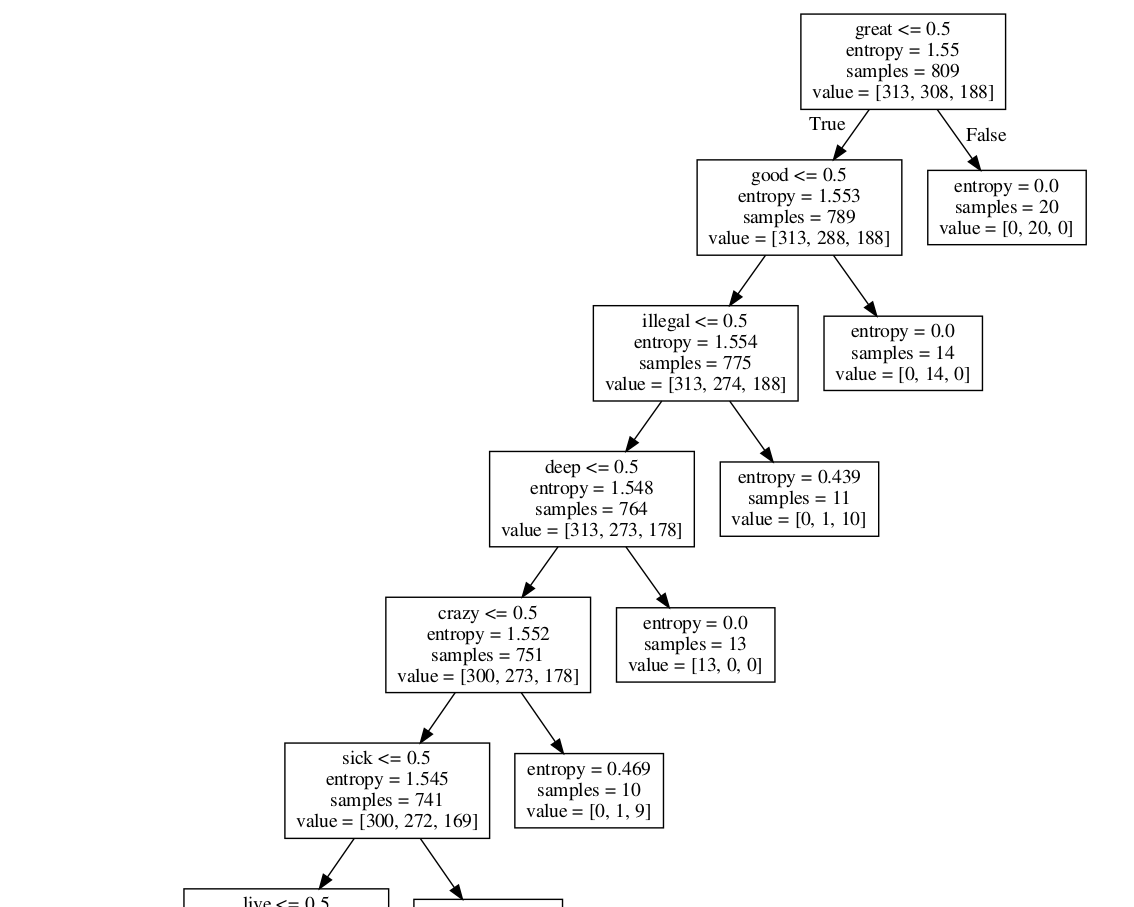
\includegraphics{../fold1_14_1.png}
\caption{}
\end{figure}

\begin{itemize}
\tightlist
\item
  Fold 1: max\_depth = 6, min\_samples\_leaf = 1
\end{itemize}

\begin{figure}[H]
\centering
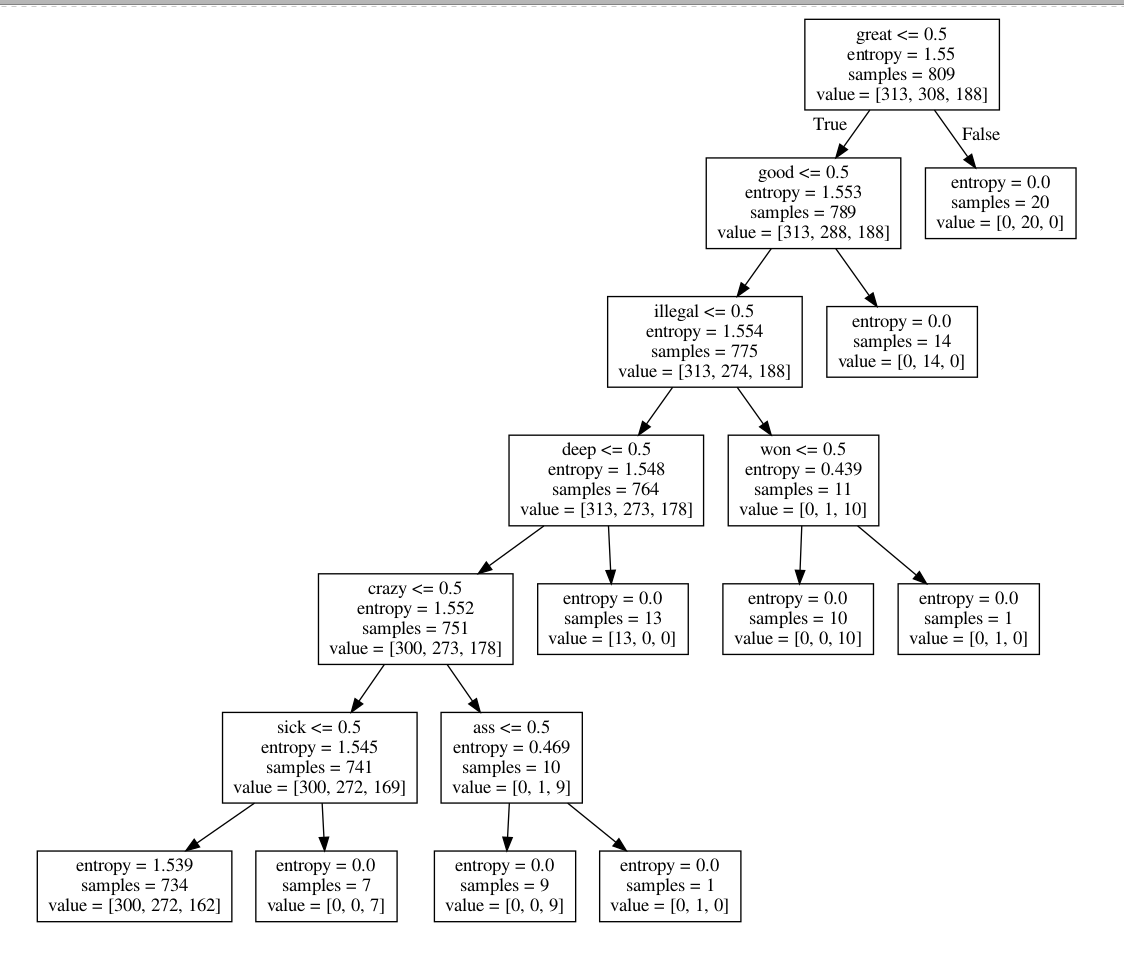
\includegraphics{../fold1_6_1.png}
\caption{}
\end{figure}

\begin{itemize}
\tightlist
\item
  Fold 5: max\_depth = 13, min\_samples\_leaf = 1
\end{itemize}

\begin{figure}[H]
\centering
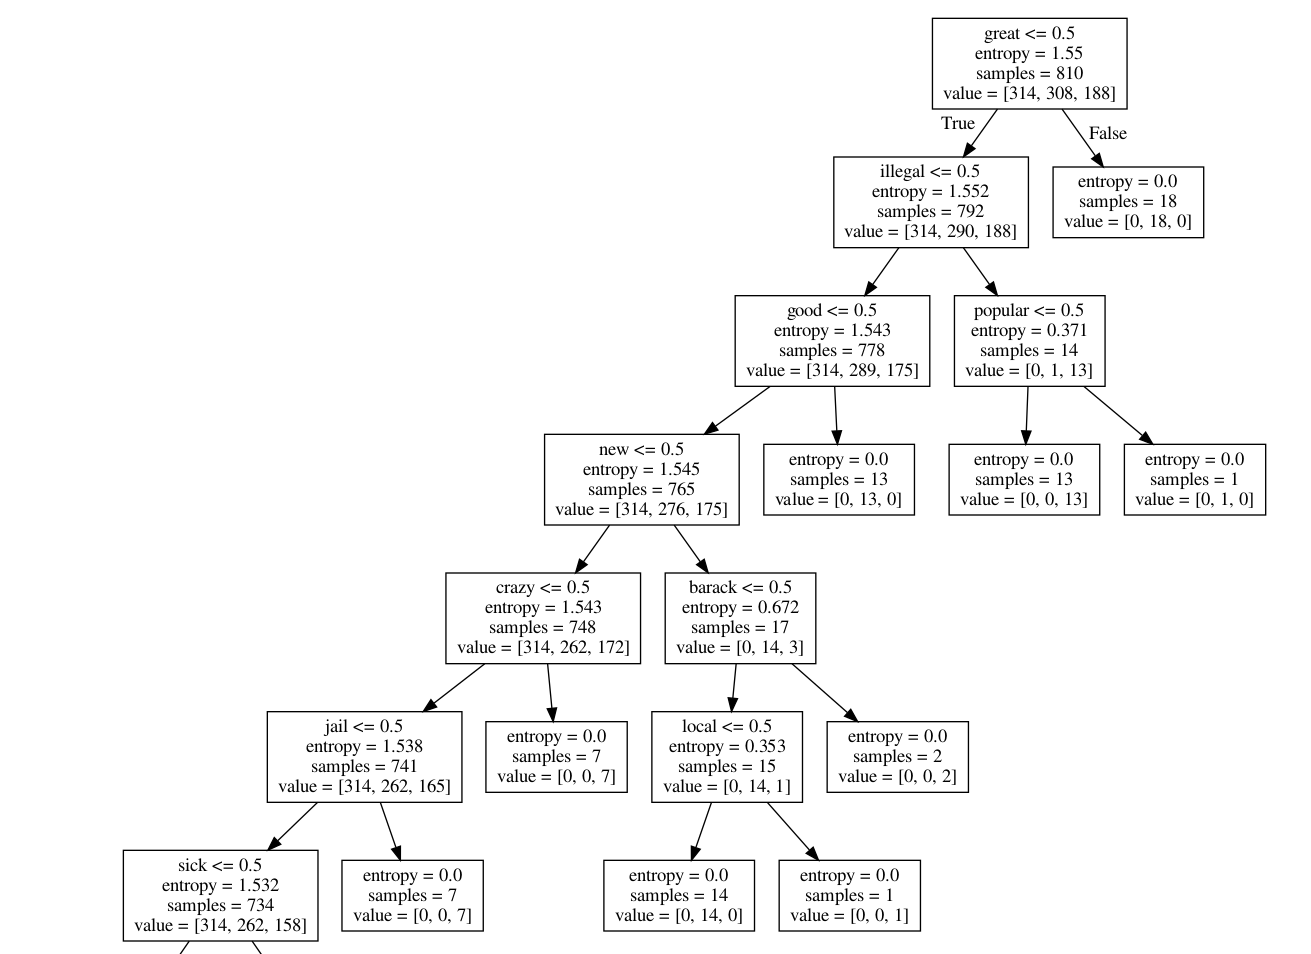
\includegraphics{../fold5_13_1.png}
\caption{}
\end{figure}

\begin{itemize}
\tightlist
\item
  Decision Trees of different combination of max\_depth and
  min\_samples\_leaf and different folds share some similar features,
  for instance:

  \begin{itemize}
  \tightlist
  \item
    \(great \le 5\) is the root node of all the sampled trees here
  \item
    \(illegal \le 0.5, good \le 0.5\) also appears in all sampled trees
  \item
    \(crazy \le 0.5, deep \le 0.5\) appears in not all but also more
    than 1 tree
  \end{itemize}
\end{itemize}

    \subsubsection*{3) discuss the results (e.g., the best combination of
max\_depth and
min\_samples\_leaf)}\label{discuss-the-results-e.g.-the-best-combination-of-max_depth-and-min_samples_leaf}

    To summarize, when
    
    \(maxDepth \in [1,15], minSamplesLeaf \in [1,5]\)
\[maxDepth= 14\]

\[minSamplesLeaf = 1\]

or
\[maxDepth= 13\]

\[minSamplesLeaf = 1\]

are probably the optimal choices since in the 5 fold cross validation,
these combination reach: -
\begin{itemize}
	\item  14, 1
	\begin{itemize}
		 \item the highest f1 score in fold3 and
		fold4 
		\item the highest precision score in fold3 
		\item the highest recall score
		in fold3 and fold4 
	\end{itemize}
\end{itemize}
\begin{itemize}
	\item 13, 1
	\begin{itemize}
		\item the highest f1 score in fold2 and fold5 
		\item the highest precision score in fold5 
		\item the highest recall score in fold5		
	\end{itemize}
\end{itemize}
 
    % Add a bibliography block to the postdoc
    
    
    
    \end{document}
